\chapter{Research approach\label{methods}}

This chapter will describe the research goal, questions and methods used. Additionally, the selected tools and scope of the research is specified. The process and iterations of the artifact are provided in this chapter that is used to collect data to be evaluated. Furthermore, the evaluation process is represented in this chapter.

\section{Research goals}

The objective of this research is to find answers to the research questions below. The research questions will help to understand the current situation of web accessibility and how web accessibility is evaluated. Based on findings of the literature review we can identify if there is potential in Generative AI when assessing accessibility of a web page. 

The research questions for the thesis are the following:

\begin{itemize}
    \item \textbf{RQ1.} What are the limitations of web accessibility evaluation tools in assessing compliance with Web Content Accessibility Guidelines (WCAG)?
    \item \textbf{RQ2.} How well does Generative AI assist to address these limitations?
\end{itemize}

The primary goal is to evaluate the capabilities of Generative AI in the scope of web accessibility evaluation, forming a tailored prompt that is the demonstrated and empirically evaluated artifact in this study. Research Question 1 (RQ1) pinpoints relevant challenges within web accessibility evaluation. Subsequently, to answer Research Question 2 (RQ2) we create an artifact in the form of a prompt. A prompt is set of instructions given to the Generative AI. The artifact is planned to be improved in iterations and each iteration is demonstrated and evaluated separately.

\section{Research methods}

This thesis will use a qualitative method based on an iterative manner of the Design Science Research Methodology (DSRM) \citep{designsciencemethodology, iterativedesignscience}. The aim of DSRM is to identify a problem and create an artifact to increase productiveness. \textcite{iterativedesignscience} presented the DSRM that consists of six phases as shown in Figure \ref{fig:design-science}.

\begin{figure}
    \centering
    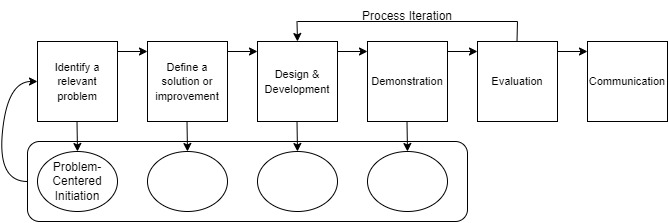
\includegraphics[width=1\linewidth]{image.png}
    \caption{DSRM Iterative Process, modelled from \textcite{iterativedesignscience}}
    \label{fig:design-science}
\end{figure}

Phase one and two, the problem identification and objective of solution, are conducted as part of the RQ1. RQ2 is answered in the iteration phase, that consists of the design \& development, demonstration and evaluation phase.

The process entry can start from any of the first four phases \citep{iterativedesignscience}. In this thesis initiation of the research was problem-centered. With multiple years of experience in web development, web accessibility is a topic I have always neglected. The problem identification and motivation started by asking myself; Why are so many web pages inaccessible even though legislation is moving forward? What needs to be done to make the web more accessible? 

With the questions in mind and very limited knowledge of web accessibility, I conducted a narrative literature review described in Chapter \ref{accessibility} of web accessibility with a legislative perspective in the EU. The review was done by delving into the \textcite{eudirective2016} and documents it referred to. In addition, Google was used to search information on web accessibility.

\section{Problem identification}

Research Question 1 is used to identify and define the objectives of a solution. Taking into account the groundwork in Chapter \ref{accessibility} from the legislative perspective and to answer RQ1 the following search string was used in the ACM Digital Library:

\begin{verbatim}
"accessibility evaluation" OR "evaluation of tools" OR "comparing tools"
\end{verbatim}

Filters applied were: Research Article and Publication Date between 2019 - 2024 to find currently relevant publication within the field. 

A total of 150 research articles were found in ACM Digital Library. Found papers were selected based on their title and abstract. An inclusion criteria was used based on if either title or abstract mentioned comparing tools, the EU Directive or the WCAG guidelines. Exclusion criteria was used if the paper title or abstract had mentioned one of the following: specific disability, specific technology, mobile accessibility or the study was conducted in a country. A snowballing method was used to identify the most commonly referred papers that are also used in this thesis as references. Additionally, found researches were searched for individually by name to find relevant literature.

The solution needs to be useful for web accessibility specialists when they are conducting their accessibility evaluation. As I have utilized Generative AI in my work as a developer, the idea to use Generative AI for web accessibility evaluation formed during the problem identification phase. Additionally, some success criterion are context based and evaluation for conformance depends on the evaluator. The goal is to build and evaluate a proof of concept for an AI assistant in web accessibility evaluation that could be incorporated into a semi-automated accessibility evaluation tool.

\section{Selected tools and scope}

The Generative AI selected for this thesis is a Large Language Model (LLM) ChatGPT 3.5 by OpenAI. Selection criteria for ChatGPT is based on the popularity of the tool in research and the tool being free to use \citep{ouyang2023llm, white2023prompt}. In this thesis, ChatGPT will be used to test the 2.4.2 Page Titled success criterion. Page Titled success criterion was chosen for this thesis as the success criterion requires manual evaluation from an accessibility expert based on context of the web page. Additionally, the success criterion has ACT rules provided by the W3C that can be used as test cases and is categorized in A-level of accessibility. 

ChatGPT 3.5 will be prompted through their web page user interface, chat.openai.com, that has training data until January 2022. Each prompt will be opened as a new chat to ensure that the conversation does not affect the outcome. 

The Page Titled success criterion is helpful for users using screen readers to identify the page without the need to delve into the page content \citep{wcag_page_titled}. To meet the success criterion on a web page a descriptive title has to be provided in the HTML source code. 

There are two helpful techniques described in the WCAG documentation for success criterion 2.4.2 to help achieve conformance, H25 and G88. Technique H25 is HTML specific and requires the <title> tag to be in place. The G88 technique is informal on how to provide a descriptive title that should describe the content of the page \citep{g88}. To test for this technique, the page has to have a title, the title has to be relevant to the content and the page content should be identifiable solely based on the title.

To help accessibility evaluation tool and methodology developers, an ACT rule has been made with examples on how to evaluate if a page title is descriptive \citep{act_rule_g88}. The ACT rule contains test cases on how tools should interpret pass and fail criteria when checking conformance. 

\section{Iteration phases}

The design \& development, demonstration and evaluation phases are used to answer RQ2. Details found in Chapter \ref{accessibility_evaluation} literature review is used to identify limitations in current accessibility evaluation tools and methodologies. Goal is to find out if Generative AI could be prompted in a way that could recognize accessibility issues. 

As a basis for the prompt, a Zero-Shot prompting method will be used. Zero-shot prompting means that no task specific examples are provided within the prompt that would guide the LLM on how to accomplish the task correctly.

Persona pattern and context manager pattern techniques from \textcite{white2023prompt} on AI prompting will be used when constructing the artifact. A prompt is a set of instructions given to the LLM to ensure specific output. Persona pattern is used to emphasize the topic of discussion, while the context pattern is used to specify the context of the input to take into account. As generalization is important for the artifact \citep{design_science_eval}, techniques of the template pattern is utilized to some extent to ensure that the artifact could be used for multiple success criteria in the WCAG related to context evaluation.

To test the artifact in each iteration, the test cases in \textcite{act_rule_g88} are used and evaluation of output is done using these test cases. An example code snippet for an ACT rule of a descriptive web page title based on context \citep{act_rule_g88}:

\begin{verbatim}
<html lang="en">
 <head>
  <title>Clementine harvesting season</title>
 </head>
 <body>
  <p>
   Clementines will be ready to harvest from 
   late October through February.
  </p>
 </body>
</html>
\end{verbatim}

These examples will be main input that the LLM should evaluate for accessibility. There are seven test cases in total, which of three should pass, three should fail, and one is inapplicable. P1, P2 and P3 are annotated as the passed test cases, failures are annotated as F1, F2, F3. As last, the only inapplicable is annotated as I1.

Inapplicable in this test example is defined that there are no applicable HTML nodes that contain a title element. The title element is part of an Scalable Vector Graphic (SVG) and provides an accessible name for the SVG rather than the whole site.

\subsection{Initial iteration}

The design of the first iteration prompt uses the persona and context pattern. The procedures in \textcite{g88} under section "Tests" is used as base rules. These rules are given in the prompt to specify the context and actions for the LLM. The expected result is that all of these three rules are true. In addition, the special case in accessibility support regarding HTML code from \textcite{act_rule_g88} is added to the ruleset. However, as WCAG is technology agnostic, the wording "document" will be changed to "web page" reflecting the style of other rules provided in the prompt. For persona, the "Web accessibility specialist" will be used, as it is a title used by \textcite{web_accessibility_specialist} that is a known accessibility organisation providing certificates in web accessibility.

The initial design of the prompt:

\begin{quote}\label{first_iteration}
From now on, act as web accessibility specialist. Pay close attention to web accessibility details of any web page that we look at. Provide outputs that a web accessibility specialist would regarding the code.

Your task is to check if the following web page conforms with the 2.4.2 Page Titled success criterion.
When analysing the following web page, only consider given web accessibility rules.

Within web page:

\textit{<ACT Test case>}

Please consider given web accessibility rules:

\begin{enumerate}
    \item Check that the Web page has a title
    \item Check that the title is relevant to the content of the Web page.
    \item Check that the Web page can be identified using the title.
    \item This rule assumes that browsers only recognize the first title element if multiple title elements are present in the web page. Testing shows that this in general is the case. Therefore the scope of this rule is limited to only checking the first title element in a web page.
\end{enumerate}

Does the web page conform with given web accessibility rules?
\end{quote}

\subsection{Second iteration}

A second iteration is done based on the perceived problems found when evaluating the output of the first version of the artifact. However, test cases will not be changed, even though the outcome indicates that the P2 and F2 test cases with multiple titles stating that \textit{"First title is incorrect"} and \textit{"Second title is ignored"} may have an effect on the outcome.

To improve accuracy of the output the Zero Shot Chain of Thought prompt method presented by \textcite{kojima2023large} will be used. In addition, the fourth rule, that is actually an accessibility support statement in the WCAG \textcite{act_rule_g88} document, will be added partially as part of the prompt before the rules. The accessibility statement being last appears to affect the outcome for other rules when there are multiple title elements present in the test cases. Moreover, the LLM is explicitly given a task to evaluate the web page based on the 2.4.2 Page Titled success criterion, therefore the question at the end of the prompt will be removed and the wording "Let's go step by step" demonstrated in \textcite{kojima2023large} will be added to hopefully increase usefulness, accuracy and consistency.

\section{Evaluation metrics}

Evaluation in DSRM is outcome based \citep{design_science_eval}. The output of the LLM is artificially produced text that will be evaluated as an entirety, taking into account the perceived usefulness of the output. Perceived usefulness as an evaluation metric is used in user acceptance of systems \citep{perceived_usefulness}. It is based on a persons subjective opinion on that using the system would enhance the effectiveness and productivity of the persons task. Subsequently, on each iteration, the LLM output will be evaluated accuracy and consistency. Accuracy and consistency of the output needs to be evaluated as current LLM's are non-deterministic \citep{ouyang2023llm, power_determinism}.

The artifact will be evaluated based on generalization at the end of the last iteration. The generalization of the artifact will be evaluated to see if the artifact could be utilized for other ACT rules that evaluate similar context based success criteria. For example, currently proposed ACT rules "Heading descriptive" or "Link descriptive".

The evaluation of usefulness in more detail will consist of how relevant and helpful the output is to the user. To evaluate usefulness, the output of the LLM will be evaluated with following characteristics: 

\begin{itemize}
    \item provides suggestions for improvement when applicable
    \item provides logical reasoning on steps it used to evaluate
\end{itemize}

However, the artifact will not explicitly ask for improvement, as final evaluation should be done by the evaluator. The perceived usefulness will be evaluated by the thesis writer.

Accuracy is evaluated based on the seven pre-defined test cases provided by W3C in \textcite{act_rule_g88}. An outcome of the overall compliance is expected from the LLM based on the rules provided in the input artifact. A passed outcome means that the test case meets all provided rules, a failed means that it partially meets the rules \citep{act_rule_g88}. In regards of inapplicable test case, the accuracy cannot be determined. In addition, consistency is evaluated by executing the same input and evaluating how often it provides perceivable identical answer in form of accuracy. 

